%
% The points that I want to cover are the following:
%
% \begin{itemize}
%   \item Building the network from the bioinformatics data and clustering.
%   \item Manipulation of the network: translation and scaling.
%   \item Locomotion and ergonomics used in the VR environment.
%   \item Changing from the blood network to the biopsy network and viceversa.
%   \item Filtering genes in the network using gene sets that represent signatures of cellular pathways which are often dis-regulated in cancer.
% \end{itemize}

%In order to explore the network, several features have been implemented with the purpose of enhance the experience of the visualization process. For example the user has the possibility to move around the network by teleporting to a different place. It is also possible to translate the network and scale it, allowing the user have a better view of the data. The user can also point at a node using the controller to show the name corresponding to that gene or node. Another feature is about entering into a menu where the user can filter the network according to gene sets that represent signatures of cellular pathways which are often dis-regulated in cancer. And finally it is possible also to switch the network from a blood dataset to a biopsy dataset and viceversa.

%The genes nodes in the network and are represented as squared dots and the relationships are represented with lines between them. In Figure \ref{fig:bignet_vr} we can see an example of the application running.

BigNet VR is a virtual reality application for the interactive visualization of large-scale networks in a 3D space. The network is represented using nodes and connections between them. In order to explore and visualize the data in BigNet VR, the user can walk around the 3D environment, scale the network, translate it to other places, filter the nodes using a user interface and also obtain detail information about the data.

BigNet VR works with a dataset that contains the information of the nodes and relationships that make up the network. We can load the dataset into the application and then run it using a HMD (Head Mounted Display) for VR. Finally we can explore the network and interact with it to visualize the data.

The implementation of BigNet VR is carried out in Unity, a cross-platform game engine. This software is used for a wide range of applications, especially for the development of videogames in 3D and 2D, VR applications and engineering solutions. The programming language used to develop the application inside Unity is C\#. We also used VRTK, a VR toolkit to build VR solutions in Unity. As for the VR hardware, we used an Oculus Quest headset. This type of headset is an oll-in-one HMD, which means that it doesn't need to be connected to a PC to run an application, it can be run inside the hardware of the headset itself. However during the development process, the headset needs to be connected to the PC and the application can be run and tested directly from Unity.

For this chapter we will use dataset examples from MIxT to illustrate the concepts that we will talk about. MIxT is a web application that is used for the visualization of bioinformatic data\cite{fjukstad_dumeaux_olsen_lund_hallett_bongo_2017}\cite{dumeaux_fjukstad_interactions_tumor_blood} and the datasets used here contain genetic information about a woman with breast cancer. There are in total 2 datasets; the first one is from a blood sample and the second one is from the tumor sample. In Figure \ref{fig:bignet_vr} we can see an example of the application running using the blood dataset from MIxT.

\begin{figure}[h!]
    \setlength{\tempheight}{15ex}
    \centering
    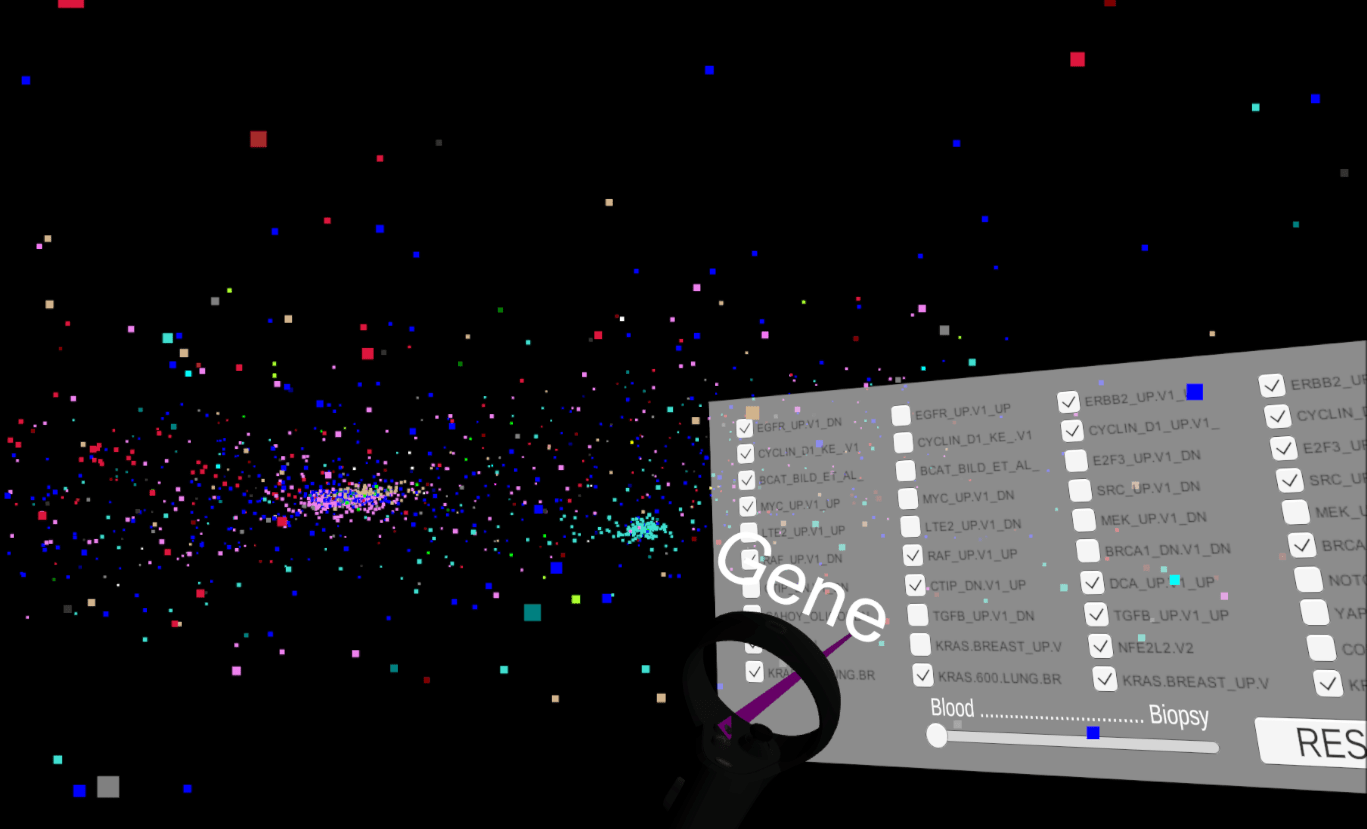
\includegraphics[width=\textwidth]{bignet_vr}
    \caption{BigNet VR. Example of the application running on a Oculus Quest.}
    \label{fig:bignet_vr}
\end{figure}

\section{Interaction with the network}
Virtual reality headsets offer a rich inmmersive experience. It's not only about inmersing the user into a 3D environment, but also giving the user the possibility to interact with the environment itself. This makes it possible to build complex VR applications where the user can do almost anything in a virtual world. Some examples of what is possible to do in virtual reality is for example moving around, grabbing objects, interact with the environment using your hands or virtual tools, 2D interfaces and menus, etc. In this section we will explain the techniques that we have implemented to visualize and interact with the network and make the most of VR. These techniques correspond to how the user can move around in the network and how the user can visualize the data.

Oculus Quest is an all-in-one VR headset and so it doesn't need a PC nor wires to run the applications. Apart from the headset, it comes with 2 controllers; one for each hand. These controllers have inputs as buttons, thumbsticks and triggers that can be used to activate actions in the VR application. We have used some of these inputs available in the controllers in BigNet VR and mapped them to different actions that allow the user interact with the network and the environment. In Figure \ref{fig:oculus_quest_inputs} we can see which actions correspond to each input from the controllers. We will explain now how we implemented the system and the different methods that we have used for the data visualization.

\begin{figure}[h!]
    \centering%
    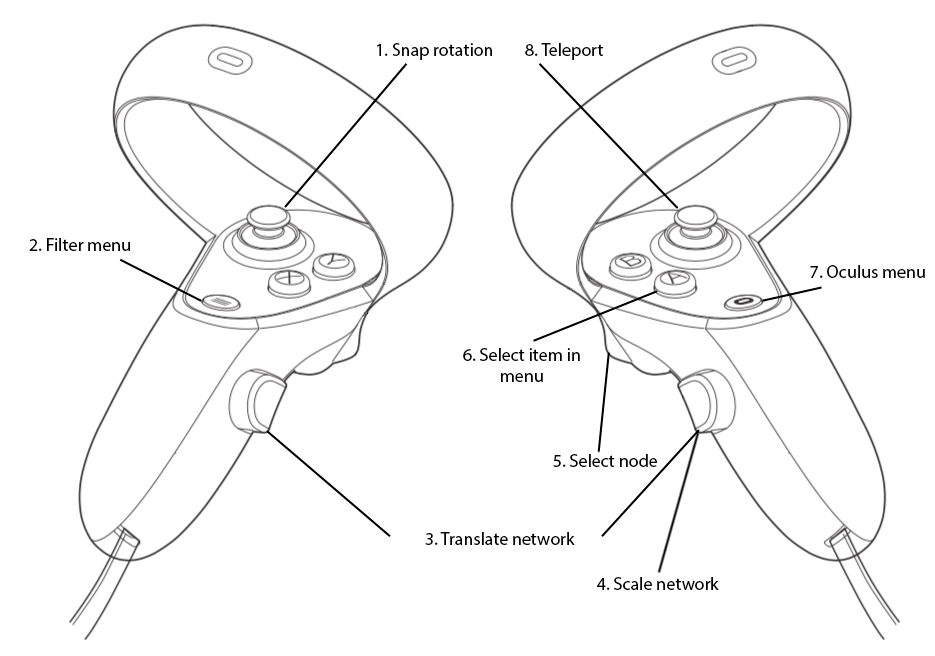
\includegraphics[width=\textwidth]{oculus_quest_inputs}
    \caption{Mapping of the Oculus Quest controllers for the different actions implemented in BigNet VR: 1. Snap rotation. 2. Filter menu. 3. Scale environment. 4. Translate environment. 5. Select item in menu. 6. Oculus menu. 7. Teleport. Adapted figure from Oculus developer's page\cite{oculus_inputs}.}
    \label{fig:oculus_quest_inputs}
\end{figure}%

\subsection{Implementation details}
Unity (version 2018.4.10f1\cite{unity2018}) is the software that was used to build the system. Unity is a multi-platform game engine. It is known to be easy to use and for having a big community of creators and asset designers\cite{developing_vr_unity}. Even though it is intuitive to use, it also has a low-level access for developers. As for Virtual Reality, Unity has been up-to-date with the new VR technologies thanks to professionals and amateurs in this area who have built integrations for Unity. In our case, our device is an Oculus Quest, and for this reason we use the Oculus integration for Unity\cite{oculus_unity_integration}. In addition we have used VRTK, a collection of ascripts and assets that help build VR solutions\cite{vrtk-what}. Finally, the programming language used in Unity to implement the system is C\#.

\subsection{Locomotion}
Locomotion is one of the most important ways of interaction in virtual reality experiences. It can be defined as a self-proppelled movement in the virtual world. Even though moving around is not the main goal in most of VR applications, it is an important aspect for the user's perspective in order to move the user's viewpoint in the virtual world and navigate around it.

Locomotion can have an strong influence in the user's experience. A poorly designed locomotion technique can reduce the user's immersion and even introduce motion sickness, which is related to the movement that the technique produces. HMDs like Oculus Quest allow the users to control the position and the orientation of the viewpoint by moving their heads and walking. However large virtual environments such as BigNet VR need a big physical tracked area which cannot be covered by just walking around. It is for this reason that we need to use a locomotion technique that makes it possible to move around without the having to walk\cite{locomotion_technique}.

The locomotion technique that we use in BigNet VR is called teleportation. It consists in choosing a spot on the floor were we want to teleport to. To do this the user has to move forward the thumbstick from the right controller (see "7. Teleport" from Figure \ref{fig:oculus_quest_inputs}). In addition it is possible to choose which direction the user will face once the teleportation is completed. To do this we just need to rotate the same thumbstick to the desired direction. Once the user releases the thumbstick, a black flash will be followed by the new position in the space. This black flash is very important when implementing some techniques because it prevents from producing motion sickness and disorientation.

\begin{figure}[h!]
    \centering%
    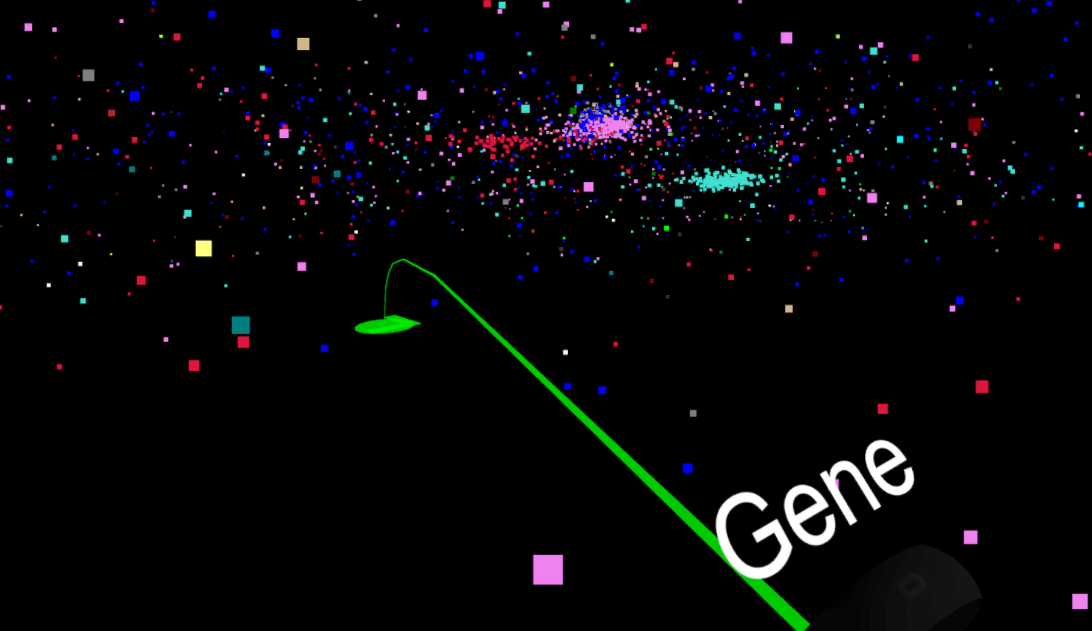
\includegraphics[width=\textwidth]{teleportation2}
    \caption{Teleportation technique. The user can use the jystick from the right controller to teleport to a different spot. To choose the spot a parabolic arc will appear.}
    \label{fig:teleportation}
\end{figure}%

In Figure \ref{fig:teleportation} we can see an example of how the teleportation technique is used in BigNet VR. A  parabolic arc is created in the 3D space with a circle representing the teleporting place. It can be seen as if we are throwing an object to the spot where we want to teleport to. The green circle includes also an arrow, indicating the direction that we will face once we are teleported.

In addition to the teleportation, we have also added the possibility to rotate to the left or to the right so that the user doesn't need to rotate the head too much. This action is triggered using the thumbstick on the left hand (See 1. Snap rotation in Figure \ref{fig:oculus_quest_inputs}). By moving the thumstick to the left side, the camera will rotate 45$^{\circ}$ to the left side, and 45$^{\circ}$ to the right side if the user moves it to the right side. A black transition is also used in this case before the rotation happens to avoid motion sickness.

\subsection{Translation of the network}
By teleporting to different places in the environment we allow the user see the network from different perspectives. However it is also interesting being able to move the network and specially move in a precise way so that the user has more control over what it is being visualized. The user might for instance be able to see the network or a specific node or cluster from above or also from below. To do this we have implemented a functionality to translate the network in the 3D space.

\begin{figure}[h!]
    \centering%
    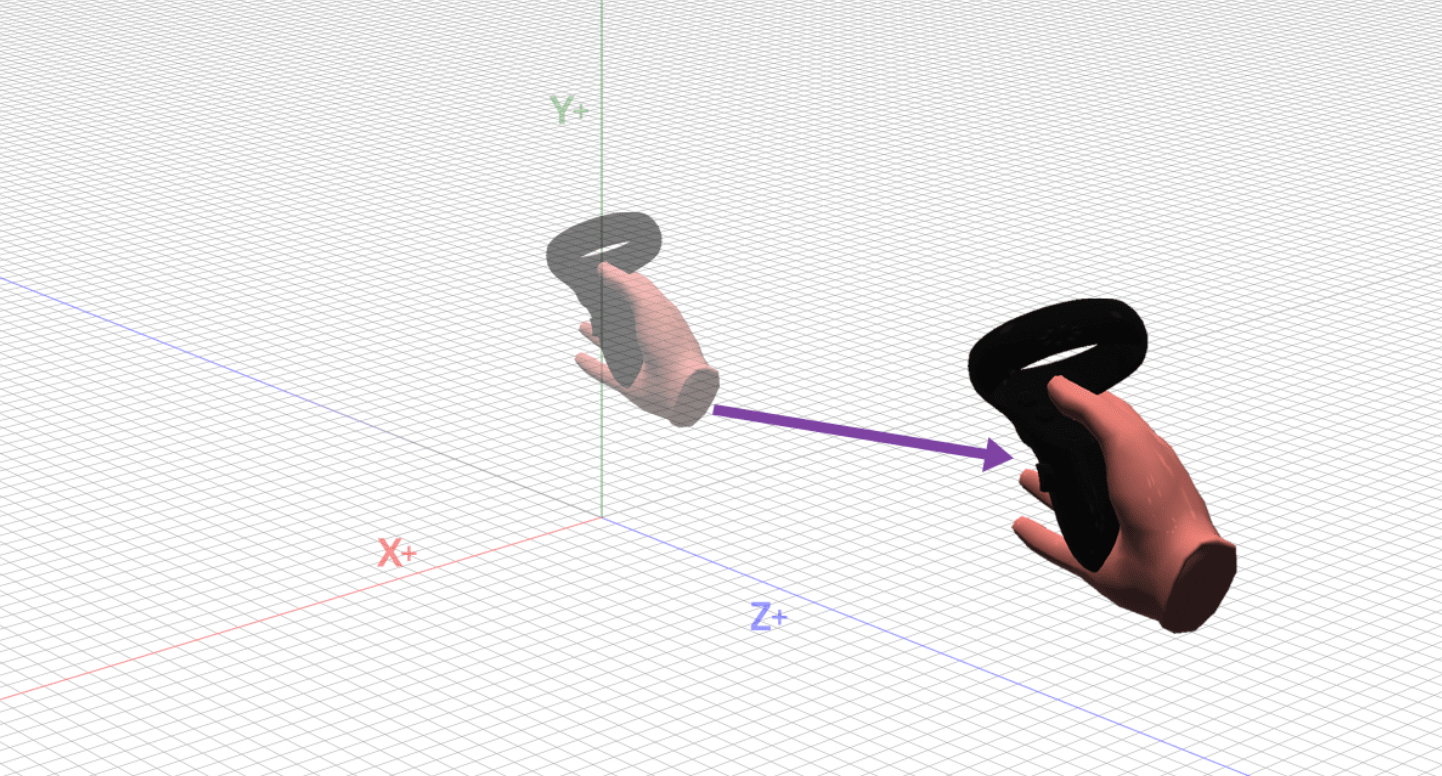
\includegraphics[width=\textwidth]{translation}
    \caption{Translation of the network functionality. The user holds the translation button on the Oculus controller and moves the hand to the direction where he or she wants the network to translate.}
    \label{fig:translation}
\end{figure}%

To translate the network in BigNet VR, the user needs to press on the hand trigger from the right controller (see "4. Translate environment" in Figure \ref{fig:oculus_quest_inputs}). Then the user needs to keep holding this trigger down and move the hand to the direction to which we want the network to move to. This intuitive approach feels like we are just pulling from a rope tied to the network and we just move it to the direction we want.


\subsection{Zooming in the network}
When exploring a big network with hundreds of nodes and several clusters, sometimes the information can be too crowded. In our example dataset that we use in BigNet VR, there are some clusters of nodes that have too many nodes close to each other and it gets very hard to visualize them properly. A way to cope with this problem is for instance by "zooming" in the part of the network that we want to explore better. We implement then a scaling functionality that makes the network bigger or smaller.

The way we implemented the zooming functionality in BigNet VR is by using the hand triggers with the name "3. Scale environment" (see the reference in Figure \ref{fig:oculus_quest_inputs}). In the first place the user needs to press and hold these triggers from both controllers and then we need to expand or contract the arms, as if we were streching out or contracting the network itself. This is also an intuitive acction to do since the user might think that we are actually stretching the network with the hands.

\begin{figure}[h!]
    \centering%
    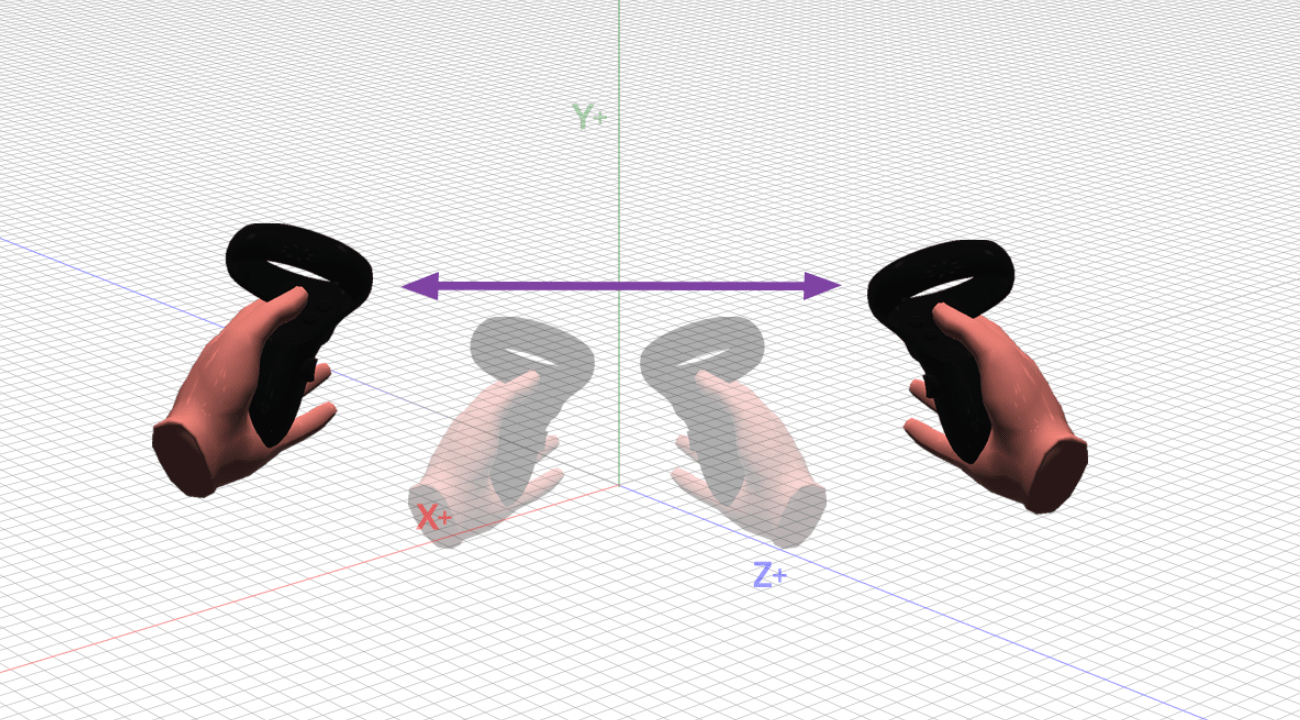
\includegraphics[width=\textwidth]{scaling}
    \caption{Zooming in the network functionality. The user can hold the scaling buttons on the Oculus controller to make the network bigger or smaller. In this example if we strech our hands outside, the network will expand.}
    \label{fig:scaling}
\end{figure}%


In Figure \ref{fig:scaling} there is a visual example of how the zooming works using the Oculus controllers. In this example the user is stretching the hands out in order to make the network bigger. The user starts in a intial position, then holds the zooming triggers from both controllers and then moves the hands out. If we wanted to make the network smaller we would do the opposite action, by contracting the hands to the inside.

\subsection{Interaction with the nodes}
BigNet VR provides also detailed information about the data that is being displayed. The user can interact with the nodes of the network to obtain information about ecah of them. In our example, the nodes represent genes and the user might be interested in knowing which gene name corresponds to a specific node. The action that we need to do to obtain the name of the gene is to point at the node that we are interested in and press the "5. pointer" index trigger on the right controller (see Figure \ref{fig:oculus_quest_inputs}). When we press this trigger, a laser pointer will appear from the virtual controller inside of the application. By pointing to a specific node with the pointer, we will get the name of that gene node that will be displayed in a rendered text.

[User figure showing how the pointer works and explain it. This part of the implementation needs to be improved.]

\subsection{Node relationships}
Finally, our dataset has information about the relationships between the nodes. BigNet VR is implemented to show also this information. Because there can be many relationships in the dataset we don't show them all at the same time. We can only see those of the nodes that are close to the user. The way that these relationships are represented is with lines between the nodes. These lines disappear once the user moves away from the nodes.

[User figure showing how the relationships are shown in the application and explain the example. This part of the implementation needs to be improved.]


\section{Building and displaying the network}
BigNet VR uses a datasets that has been created from a external source to build the network. The datasets have to be in CSV format and we need 2 datasets in total to build the network. The first one contains the information about the categories and the nodes that belong to each category and the second dataset has information about the relationships between each of the nodes.

The following diagram in Figure \ref{fig:create_network} explains in a broad way what steps we follow to build the network in Unity. We start with the 2 datasets described before, containing the data for the network. We process the dataset with information about the categories and build a particle system object in Unity, where each particle corresponds to a node. We also add to each particle a color, which is related to the category that the particle belongs to. Finally we apply a cluster algorithm using the data from the dataset with information about the relationships.

\begin{figure}[h!]
    \centering%
    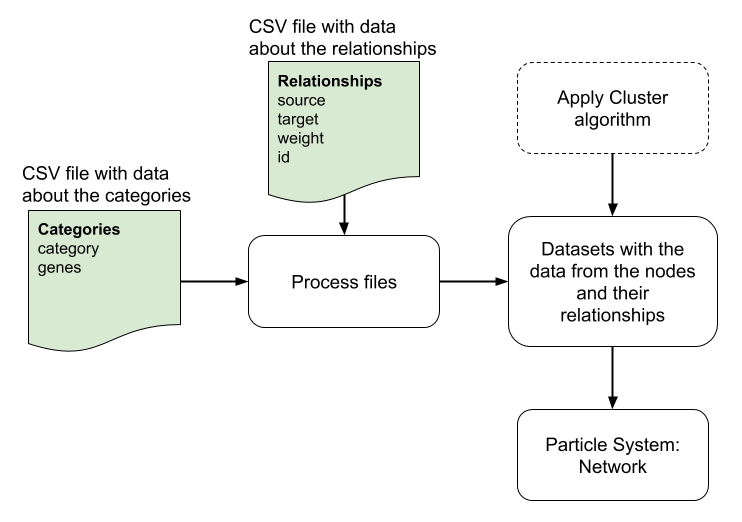
\includegraphics[width=\textwidth]{create_network}
    \caption{Diagram explaining how the network is built in Unity.}
    \label{fig:create_network}
\end{figure}%

Following our bioinformatic network example, in Table \ref{tab:categories-data} and Table \ref{tab:network-data} we show an extract of how the datasets look like. Table \ref{tab:categories-data} has the data about the nodes or genes in this case and the categories to which each node belongs to. These categories are named by colors and these color names will be used by BigNet VR to color each particle of the particle system. Then in Table \ref{tab:network-data} we have the information about the relationships. This dataset can be very extend because each row of the CSV file corresponds to a relationship between 2 nodes or genes in this case and one gene can be connected to many other nodes.

\begin{table}[h!]
\centering
\begin{tabular}{ll}
\hline
category & genes          \\
brown   & ARHGAP30 FERMT3 ARHGAP25 CD53 PLEK IRF8 DOCK2\\
cyan  & SAFB MOB3A RAB35 ABR ASCC2 CDC37 ANKFY1 GLTSCR1\\
darkgrey  & RAB40C ZNF213 ZNF263 PIGQ RHBDF1 RAB11FIP3\\
darkorange  & TCEB1 MRPL13 ENY2 MTERF3 UBE2W WDYHV1\\
\hline
\end{tabular}
\caption{Fragment of the dataset with the categories and the genes belonging to each category from the biopsy sample.}
\label{tab:categories-data}
\end{table}

\begin{table}[h!]
\centering
\begin{tabular}{llll}
\hline
source & target & weight            & id          \\
AAMP   & ARGLU1 & 0.102486209330144 & AAMP-ARGLU1 \\
ACADM  & FOXN2  & 0.107506881676173 & ACADM-FOXN2 \\
ACADM  & MBNL1  & 0.12269622045714  & ACADM-MBNL1 \\
ACADM  & PPM1B  & 0.103496640767895 & ACADM-PPM1B \\
\hline
\end{tabular}
\caption{Fragment of the dataset used to build the network relationships of the blood sample.}
\label{tab:network-data}
\end{table}

\section{Filtering information in the network}
Another feature that BigNet VR uses to improve the visualization of networks is a filtering menu. When we have huge amounts of data in large networks, it is sometimes necessary to show less or more data. By filtering the nodes we can visualize only the part that we are interesting in.


\begin{figure}[h!]
    \centering%
    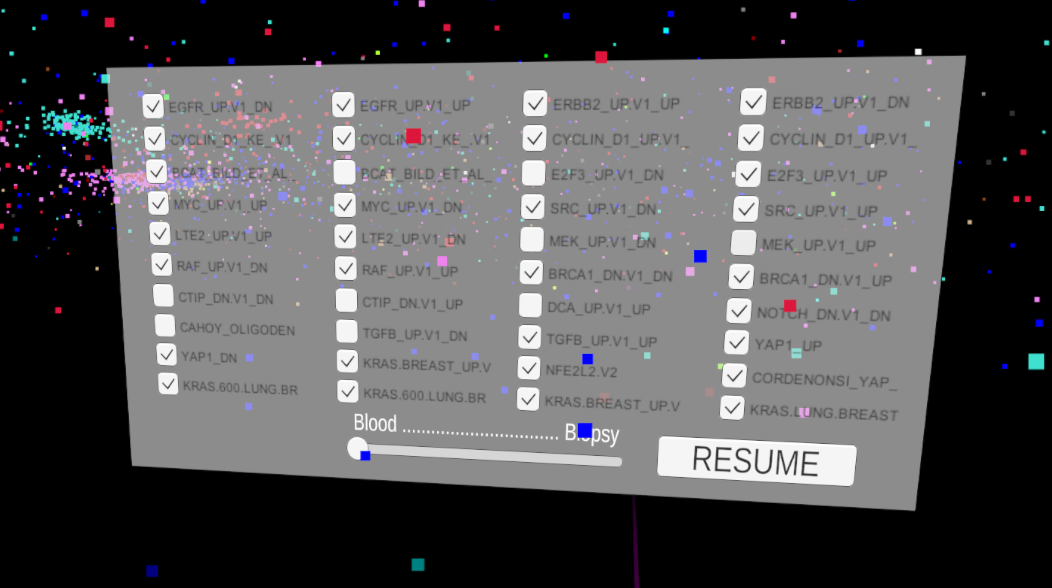
\includegraphics[width=\textwidth]{filtering}
    \caption{Filtering menu in BigNet VR.}
    \label{fig:filtering}
\end{figure}%


We have built a 2 dimensional menu in Unity, see Figure \ref{fig:filtering}, to filter the data in our example network. We use checkboxes for the filtering. From a starting point, all the boxes are checked, and if the user wants to hide a part from the visualization it is done by unchecking the box. To show the filtering menu we need to press on the menu botton from the left controller, see the "2. Filter menu" in Figure \ref{fig:oculus_quest_inputs}. The to check or uncheck the boxes we need to use the A botton from the right controller, named "6. Select item", see Figure \ref{fig:oculus_quest_inputs}.

\section{Switching dataset}
Finally BigNet VR has also the possibility to switch between datasets. This can be done in the filtering menu by pressing the menu button from the left controller and there we can see a slider UI element as in Figure \ref{fig:filtering} which we can move to the right or to the left in order to change the dataset that is being visualized. When we switch the dataset, the filters are also reset to their default state, so all of them will be checked in our example. In our bioinformatic usecase we can switch from the blood dataset to the biopsy one.
